\documentclass[11pt]{article}
\usepackage[margin=1in]{geometry}
\usepackage{amsmath,amssymb,booktabs,graphicx,microtype,xcolor,hyperref}
\usepackage[font=small,labelfont=bf]{caption}
\usepackage{subcaption}
\usepackage{siunitx}
\graphicspath{{figures/}}
\hypersetup{colorlinks=true,linkcolor=blue!55!black,urlcolor=blue!55!black}
\newcommand{\todo}[1]{\textcolor{red!70!black}{[TODO: #1]}}
\newcommand{\method}{quiet-normalized multi-lag temporal ICA}

\title{Quiet-Normalized Multi-Lag Temporal Filtering Reveals Sparse Calcium Activity in Low-SNR Whole-Field Imaging\\\large Living manuscript --- preliminary results}
\author{\todo{Author list and affiliations}}
\date{Version \today}

\begin{document}
\maketitle

\begin{abstract}
Detecting sparse calcium events in low-signal-to-noise whole-field recordings is complicated by static anatomy, spatially heterogeneous noise, and temporally persistent background intensity. We evaluated causal temporal embeddings in which each pixel was represented by its current intensity and $K$ preceding samples, then fitted symmetric InfoMax/FastICA without using event labels. A frozen $K=8$ component formed a predominantly positive, low-frequency finite impulse response (FIR) filter using nine samples from the current frame through 160 ms in the past. Robust per-pixel centering and scaling from a quiet interval, followed by positive rectification, produced visually sparse activity evidence and recovered 54 of 79 known sparse-positive occurrences with 726 candidates. A post-hoc $K=16$ diagnostic recovered 60 of 79 occurrences with 639 candidates, but was not the frozen audit operating point. The $K=8$ kernel had DC gain 2.518, peak response at \SI{0}{Hz}, and only 0.248 cosine similarity to a first difference, indicating that its primary action was temporal integration rather than differentiation. These observations motivate a testable hypothesis: much of the apparent improvement arises from the compound action of short-horizon integration, pixelwise robust quiet normalization, and positive rectification, rather than physical source separation by ICA alone. This manuscript records the result, its provenance, and the matched controls required before a stronger mechanistic or detection claim.
\end{abstract}

\section{Working claims and evidentiary status}
\paragraph{Supported by the completed run.}
A quiet-fitted multi-lag ICA component can act as a stable, positive temporal integrator; when followed by robust pixelwise quiet normalization, it yields visually sparse excitation evidence and substantial known-positive recovery. The complete three-section scientific audit passed inventory and media validation.

\paragraph{Not yet established.}
The experiment does not show that ICA recovered an independent physical neural source, that the method outperforms matched non-ICA temporal smoothers at an equal candidate budget, or that unmatched candidates are false positives. Sparse annotations define known positives, not exhaustive negatives.

\section{Data and conventions}
The source is the Spon Ca Burst hindbrain-to-tail fluorescence recording with 2,359 frames of size $340\times573$ pixels and a frame period of \SI{20}{ms}. The analyzed review interval comprises UI frames 1800--2359. It contains 79 labeled burst-specific occurrences belonging to 27 recurring ROI identities across four bursts. UI frames are one-based and inclusive; array intervals are zero-based and half-open. Coordinates use $x=$ column and $y=$ row. Labels were excluded from temporal-filter fitting and component selection and used afterward for sparse-positive evaluation and audit geometry.

\begin{figure}[t]
  \centering
  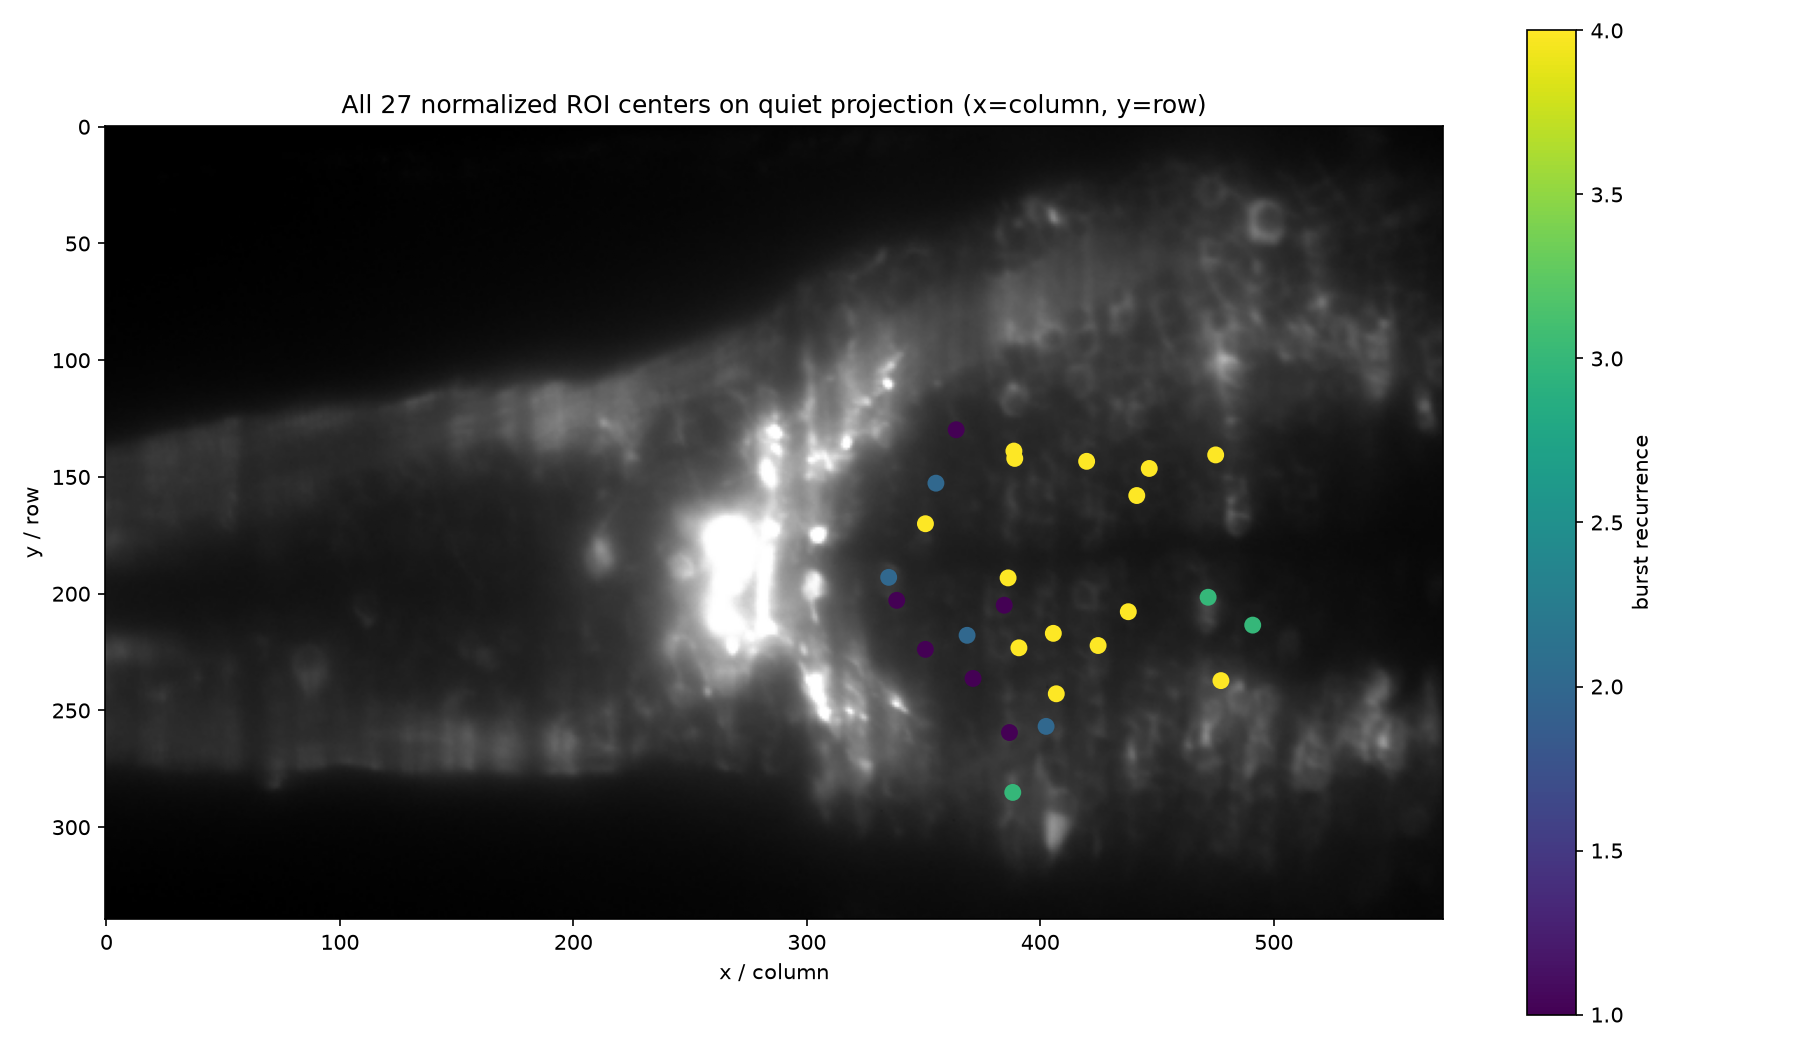
\includegraphics[width=.93\linewidth]{label_projection_overlay.png}
  \caption{Projection of the 27 recurring expert ROI identities onto the quiet-field anatomy. This preflight figure checks coordinate and frame conventions; it is not used for fitting.}
  \label{fig:projection}
\end{figure}

\section{Method}
\subsection{Causal multi-lag embedding}
At each pixel, the temporal observation vector for order $K$ was
\begin{equation}
\mathbf{x}_t=[I_t,I_{t-1},\ldots,I_{t-K}]^\mathsf{T}.
\end{equation}
Each learned demixing row was interpreted as a causal FIR kernel,
\begin{equation}
y_t=\sum_{k=0}^{K} w_k I_{t-k},
\end{equation}
rather than as evidence of independently measured physical sources. Models with $K\in\{1,2,4,8,16\}$ were fitted to 20,000 anatomy-bounded samples from the first 100 quiet review frames. Three deterministic seeds (7, 19, and 37) were used. Component selection was label-free and favored positive skew while considering derivative similarity and DC gain.

\subsection{Frozen $K=8$ FIR component}
The audit froze $K=8$ before known-label comparison. Its nine unit-norm taps were
\begin{equation}
\mathbf{w}=[0.074,0.425,0.027,0.397,0.271,0.131,0.556,0.157,0.481].
\end{equation}
All taps were positive. The component had DC gain 2.518, peak frequency \SI{0}{Hz}, first-difference cosine 0.248, second-difference cosine 0.306, and positive skewness 2.423. Seed-to-reference cosine stability was 0.900 and 0.884. Thus the selected component is better described as an uneven short-horizon temporal integrator than as a learned first-difference operator.

\subsection{Frequency-domain interpretation}
For sampling rate $f_s=\SI{50}{Hz}$, the response is
\begin{equation}
H(f)=\sum_{k=0}^{8}w_k\exp\left(-i2\pi f k/f_s\right).
\end{equation}
ICA sign and scale are arbitrary, so we orient the kernel to positive DC and use either unit-$\ell_2$ normalization (noise-gain convention) or unit-DC normalization (averaging convention). The unit-DC taps are
\begin{equation}
[0.029,0.169,0.011,0.158,0.108,0.052,0.221,0.062,0.191].
\end{equation}
The appropriate low-frequency delay is the DC-normalized centroid,
\begin{equation}
\tau_g(0)=\frac{\sum_k k w_k}{\sum_k w_k}=4.642\ \text{frames}=\SI{92.8}{ms}.
\end{equation}
The previously reported raw moment 11.689 is not a delay because the unit-$\ell_2$ taps do not sum to one. The energy centroid is 4.911 frames (\SI{98.2}{ms}), the first $-3$ dB crossing is \SI{2.543}{Hz}, and the one-sided equivalent noise bandwidth is \SI{3.942}{Hz}. Relative to DC, amplitude is 0.951 at \SI{1}{Hz}, 0.812 at \SI{2}{Hz}, 0.608 at \SI{3}{Hz}, and 0.165 at \SI{5}{Hz}.

The filter is not a monotone low-pass. Uneven taps produce response minima near 5.65, 11.44, and \SI{15.79}{Hz}, plus a secondary lobe near \SI{20.77}{Hz} with amplitude 0.486 relative to DC ($-6.26$ dB). A nine-frame boxcar has nearly the same response below \SI{3}{Hz} but much stronger rejection near \SI{20}{Hz}. Thus the learned operator can retain or reshape some fast fluctuations while integrating slow signals.

\begin{figure}[t]
\centering
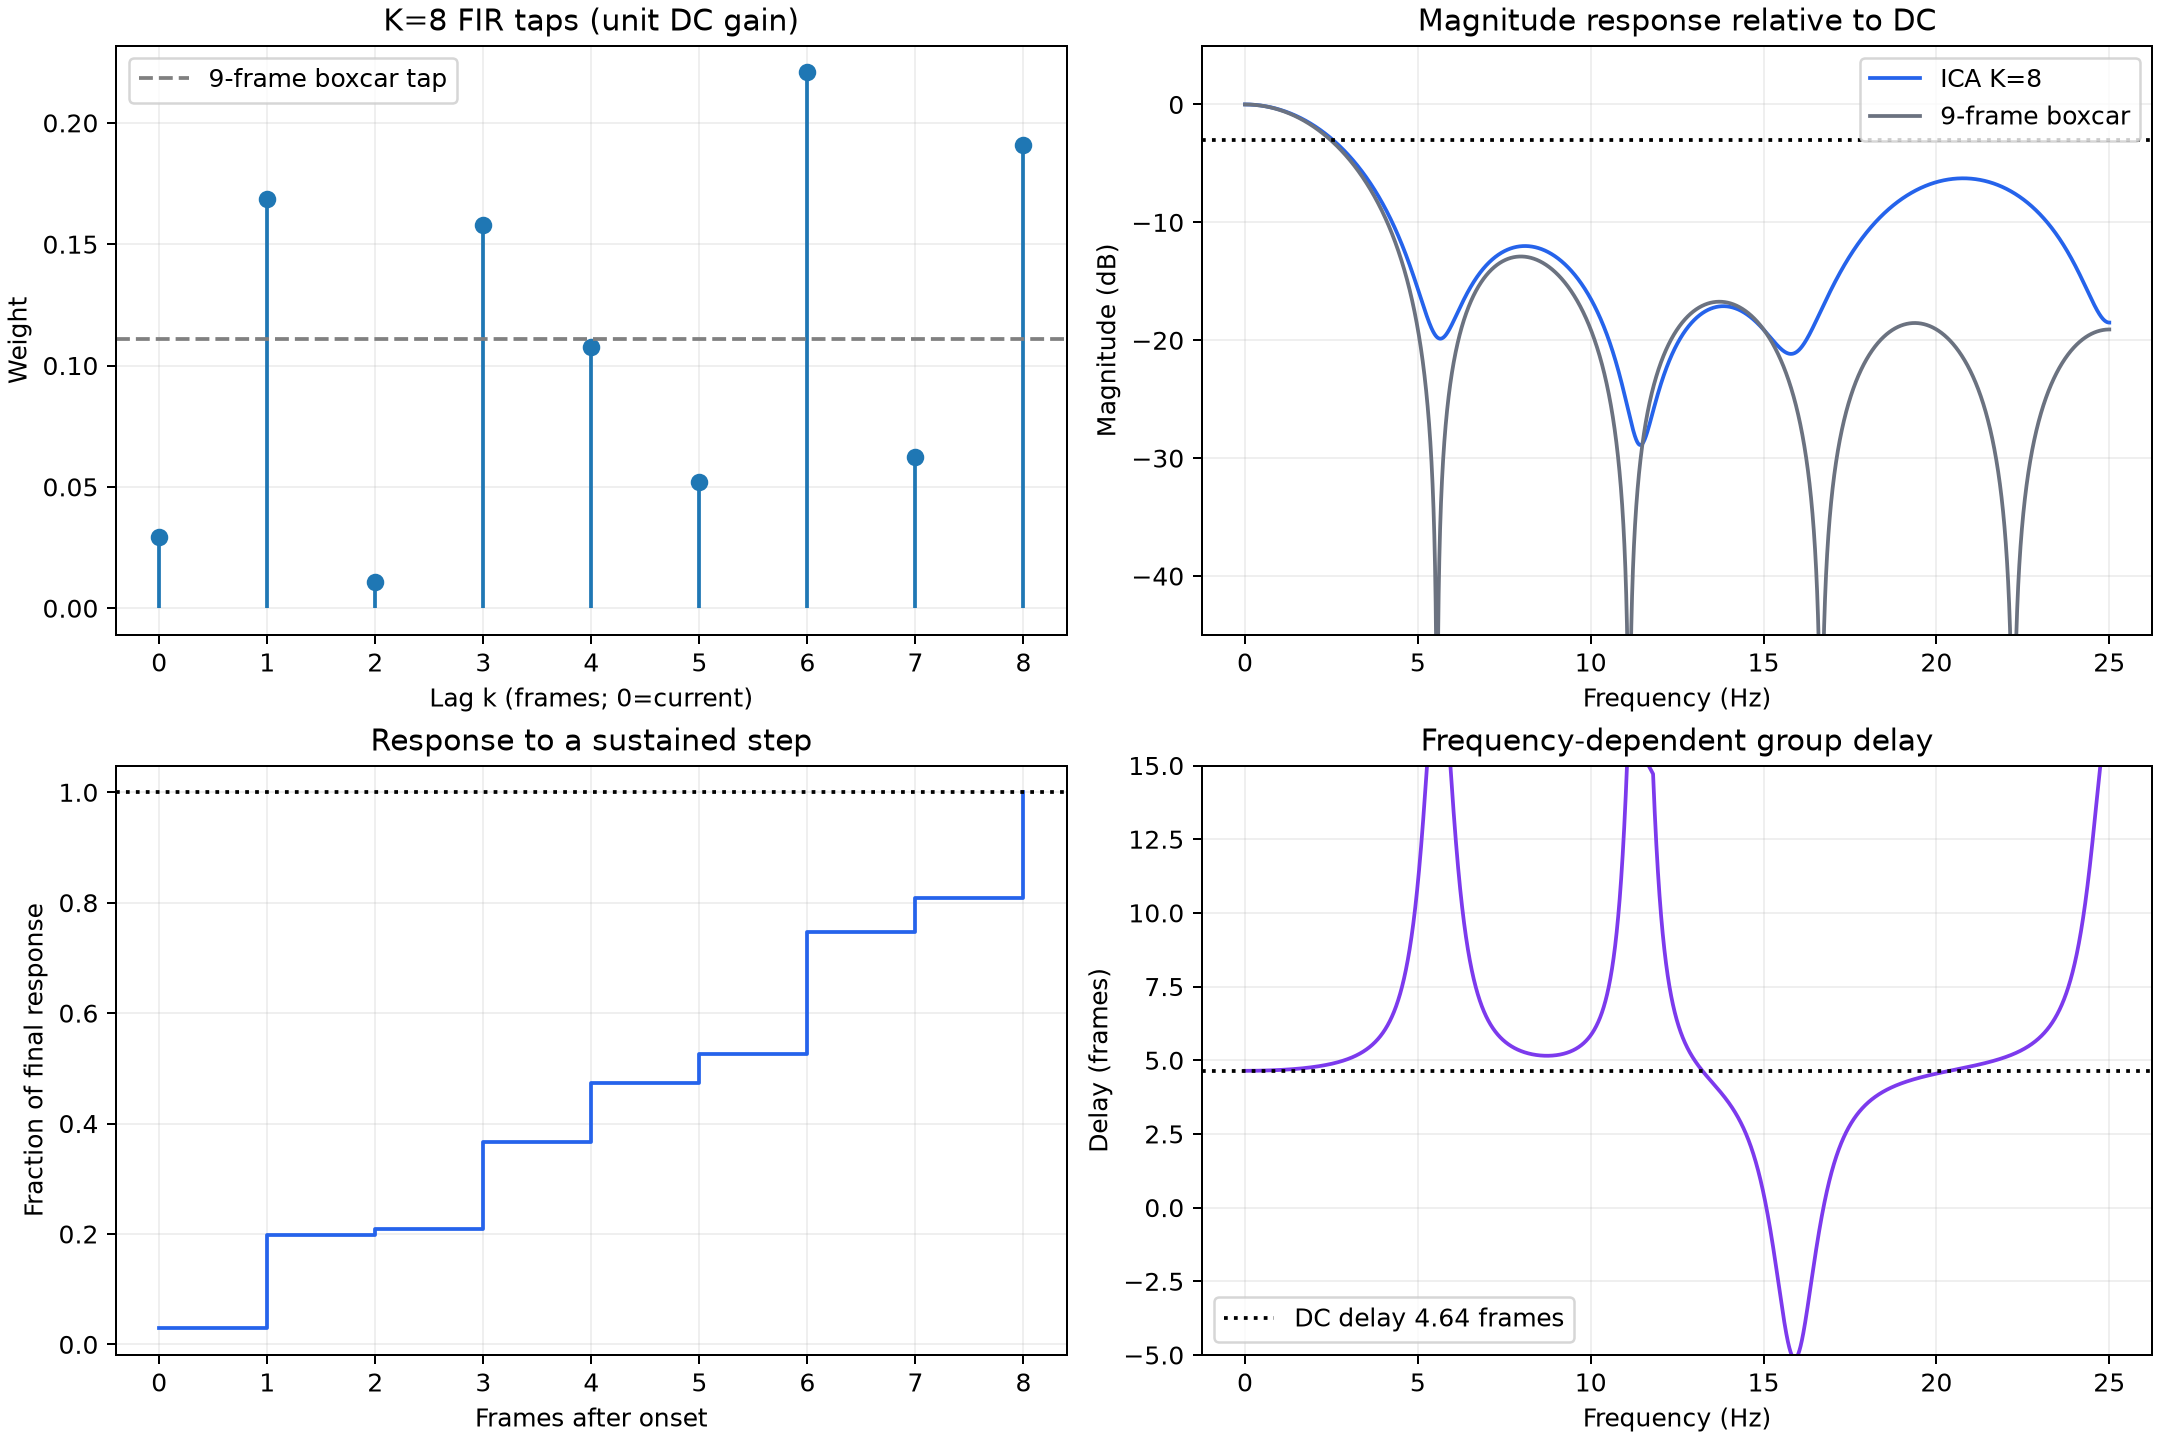
\includegraphics[width=\linewidth]{k8_fir_interpretation.png}
\caption{Time- and frequency-domain interpretation of the frozen $K=8$ kernel. Dominant low-frequency integration has approximately \SI{93}{ms} delay, but uneven taps create ripple and a high-frequency secondary lobe relative to a boxcar.}
\label{fig:k8interpretation}
\end{figure}

\paragraph{Relation to an ordinary moving average.}
The unit-$\ell_2$ $K=8$ ICA kernel has cosine similarity $2.518/3=0.839$ to a uniform nine-sample boxcar. Their normalized amplitudes differ by less than 0.02 through \SI{3}{Hz}. For unit DC gain, however, white-noise standard deviation is $\sqrt{\sum_k h_k^2}=0.397$ for the ICA kernel and $1/3=0.333$ for the boxcar. The ICA kernel therefore passes approximately 19\% more white-noise standard deviation and has larger equivalent noise bandwidth (3.942 versus \SI{2.778}{Hz}). Its current evidence does not support interpreting the uneven ICA weights as a better general-purpose smoother. The principal plausible advantage must instead come from data-adapted spectral shaping, interaction with non-white recording noise, or the downstream pixelwise quiet normalization; these alternatives require direct ablation.

\subsection{Cross-seed stability}
The three $K=8$ fits agree more strongly on low-frequency behavior than on individual taps or high-frequency rejection. DC delays were 4.642, 4.730, and 4.353 frames (87.1--\SI{94.6}{ms}); first $-3$ dB crossings were 2.543, 2.908, and \SI{2.446}{Hz}. Equivalent noise bandwidth ranged from 3.942 to \SI{5.409}{Hz}. In contrast, the Nyquist/DC ratio ranged from 0.119 to 0.410. We therefore interpret short-horizon integration and approximate delay as reproducible properties, but do not assign biological meaning to individual tap peaks or high-frequency lobes.

\begin{figure}[t]
\centering
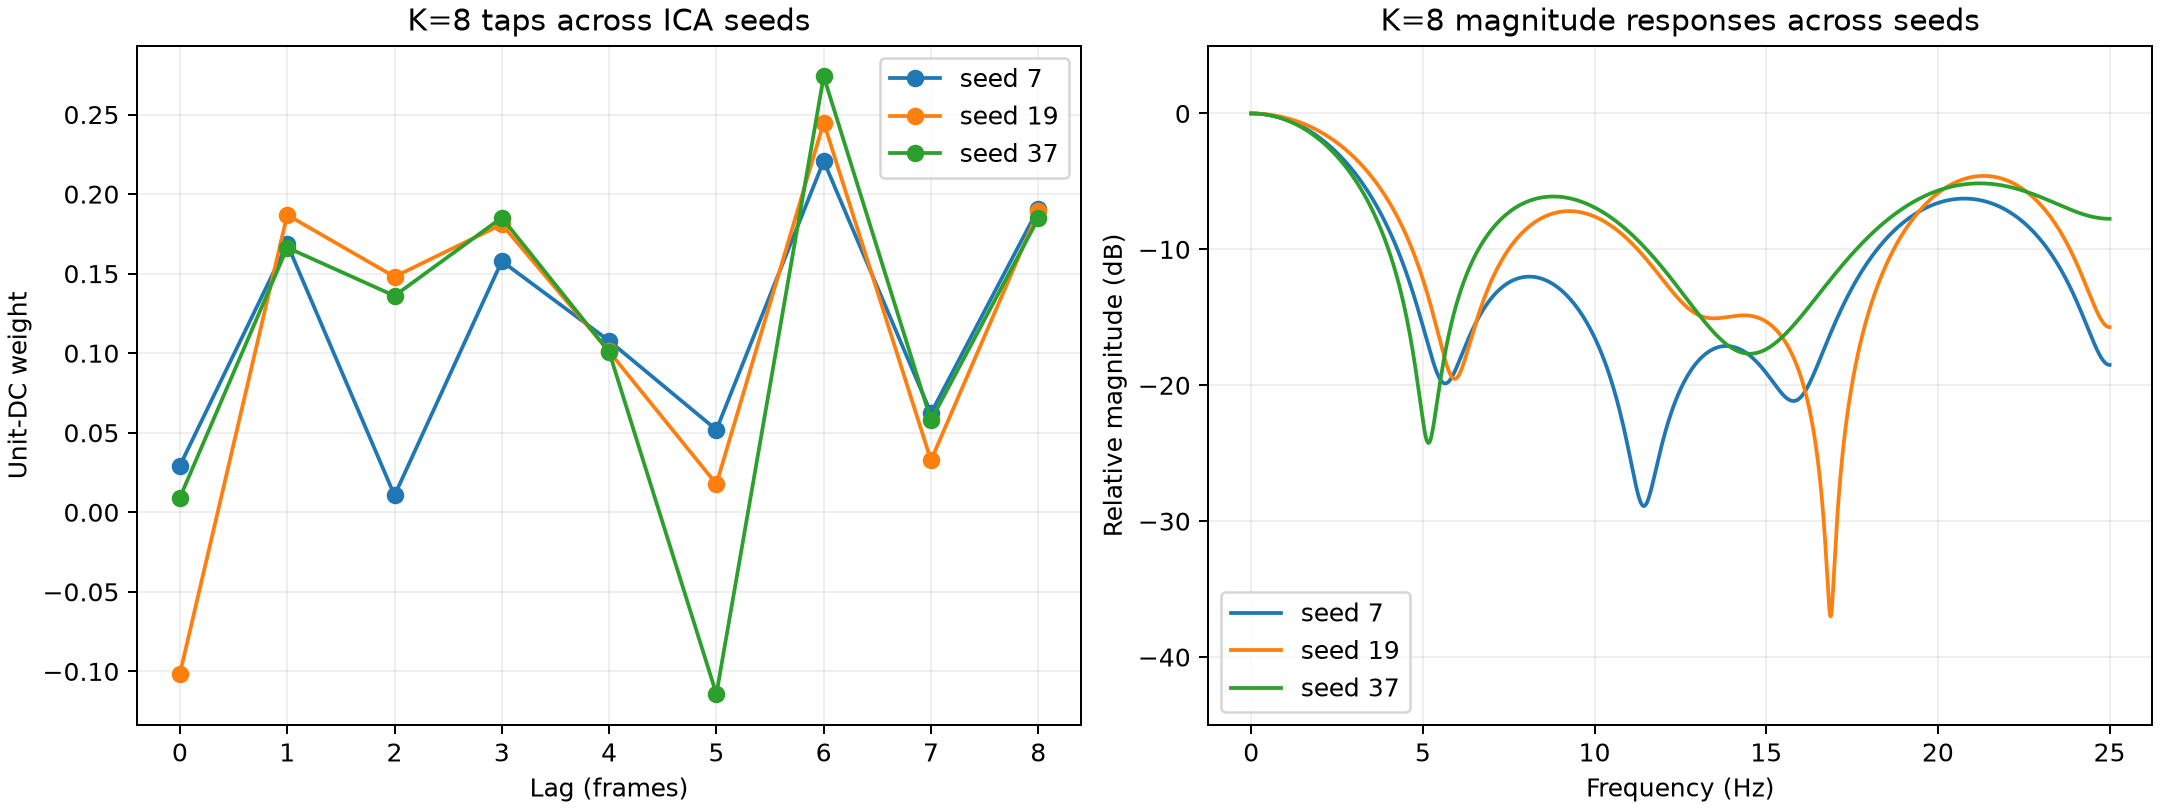
\includegraphics[width=\linewidth]{k8_seed_frequency_stability.png}
\caption{Tap and response variability across three deterministic $K=8$ ICA seeds after positive-DC orientation and DC normalization. Slow-signal integration is consistent; detailed ripple is less stable.}
\label{fig:k8seeds}
\end{figure}

\subsection{Positive quiet-standardized evidence}
For each pixel independently, we computed the quiet median $m(x,y)$ and robust scale
\begin{equation}
s(x,y)=1.4826\,\mathrm{median}_{t\in Q}\left|y_t(x,y)-m(x,y)\right|.
\end{equation}
A global lower scale floor $s_{\min}$, defined as the 10th percentile of positive pixel scales, prevented division by extremely small values. Displayed and detected evidence was
\begin{equation}
z_t^+(x,y)=\max\left(\frac{y_t(x,y)-m(x,y)}{\max[s(x,y),s_{\min}]},0\right).
\label{eq:quietz}
\end{equation}
This compound operator (i) accumulates temporally persistent brightness, (ii) subtracts stable anatomy pixel by pixel, (iii) equalizes heterogeneous quiet variability, and (iv) suppresses negative excursions. The last two operations can make the output perceptually much cleaner than the signed FIR stage without proving improved specificity.

\begin{figure}[t]
  \centering
  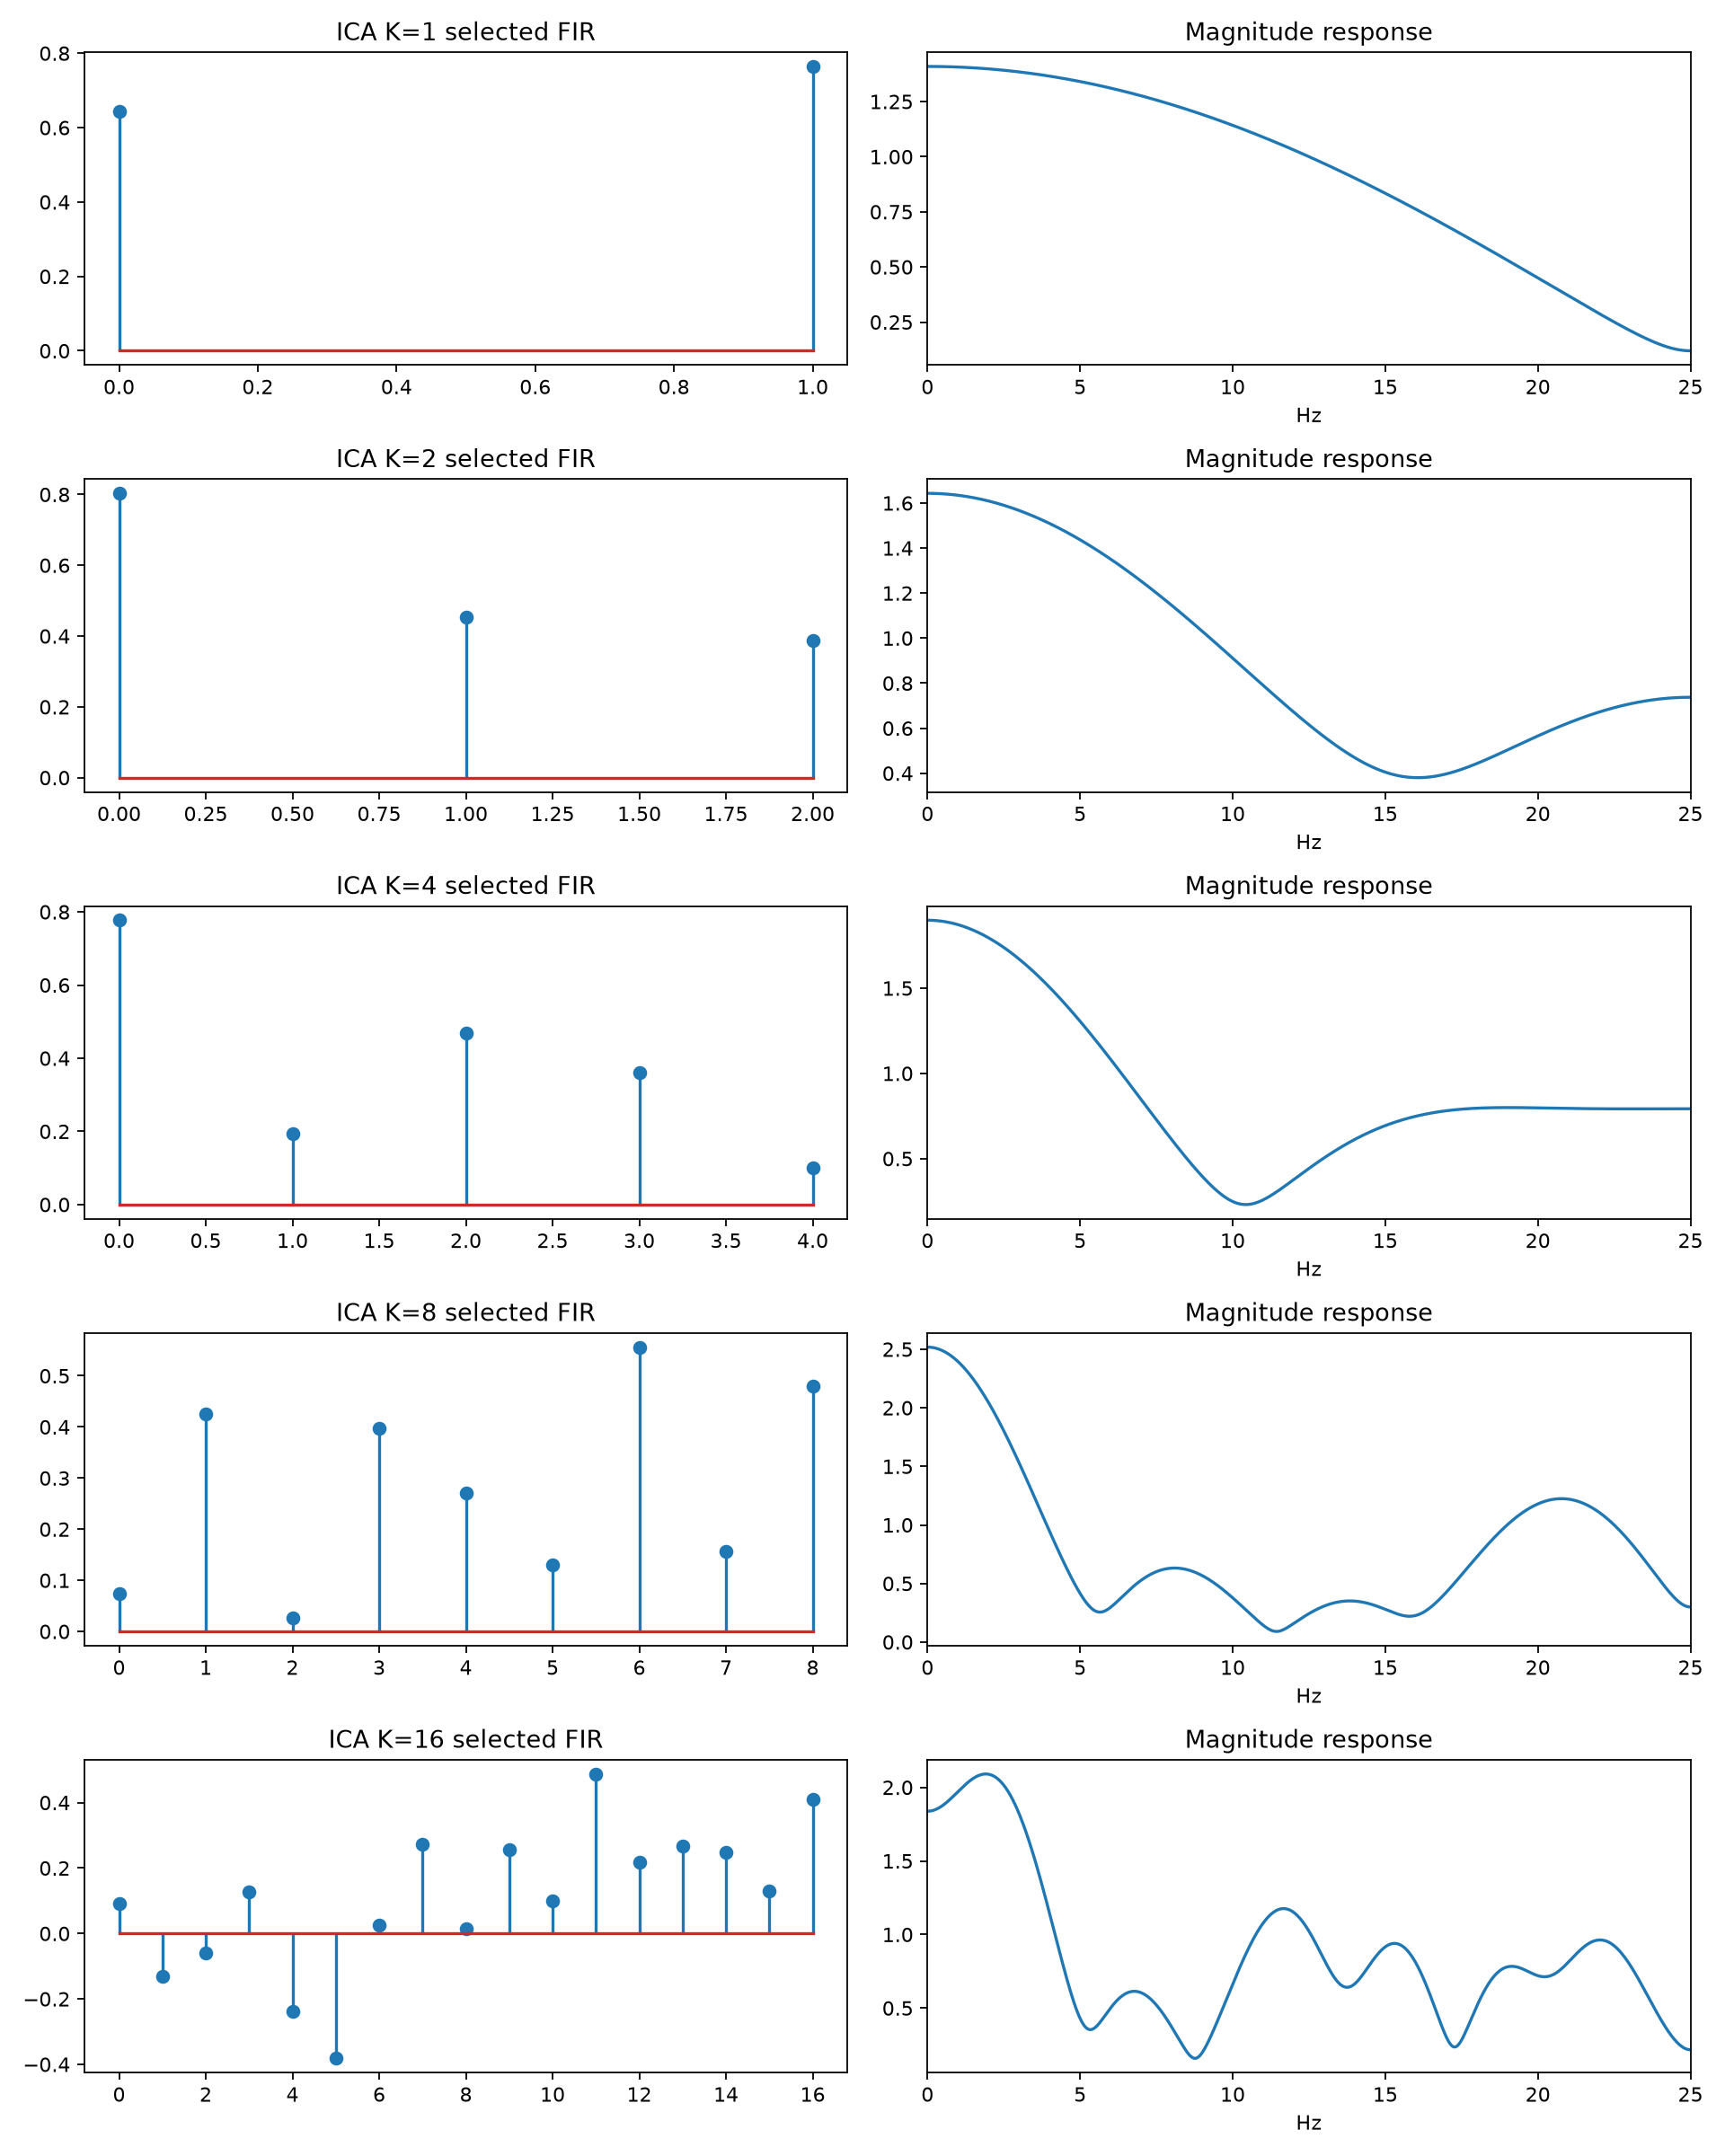
\includegraphics[width=\linewidth]{ica_kernels_and_frequency.png}
  \caption{Selected ICA FIR kernels and frequency responses over lag orders. The frozen $K=8$ component has a positive DC response and is not primarily derivative-like.}
  \label{fig:kernels}
\end{figure}

\subsection{Quiet-calibrated sparse-positive evaluation}
Positive quiet-$z$ evidence was max-pooled within each burst. Local maxima were separated by six pixels. The operating-point threshold was calibrated from local maxima in quiet windows without labels. One-to-one matching used a six-pixel radius. Unmatched candidates were retained as unknown rather than counted as negatives; consequently the study estimates known-positive recall but not precision.

\section{Results}
\subsection{Multi-lag comparison}
\begin{table}[t]
\centering
\caption{Known-positive recovery at each lane's independently quiet-calibrated operating point. Candidate counts differ and must not be interpreted as matched-budget precision. The frozen audit lane is marked with $\dagger$; the post-hoc known-label winner is marked with $\ast$.}
\label{tab:results}
\begin{tabular}{lrrr}
\toprule
Lane & Macro recall & Matches / 79 & Candidates\\
\midrule
First difference & 0.0000 & 0 & 6\\
Second difference & 0.0000 & 0 & 3\\
AR innovation, $K=1$ & 0.0000 & 0 & 6\\
AR innovation, $K=2$ & 0.0000 & 0 & 3\\
AR innovation, $K=4$ & 0.0228 & 2 & 5\\
AR innovation, $K=8$ & 0.2328 & 19 & 27\\
AR innovation, $K=16$ & 0.4171 & 34 & 69\\
ICA, $K=1$ & 0.6733 & 54 & 278\\
ICA, $K=2$ & 0.7294 & 58 & 312\\
ICA, $K=4$ & 0.7134 & 57 & 527\\
ICA, $K=8^{\dagger}$ & 0.6880 & 54 & 726\\
ICA, $K=16^{\ast}$ & \textbf{0.7559} & \textbf{60} & 639\\
\bottomrule
\end{tabular}
\end{table}

The frozen $K=8$ lane recovered 54/79 known occurrences. The post-hoc $K=16$ lane recovered 60/79, but selecting it by labeled recall makes it a diagnostic ceiling rather than the frozen model result. The very low counts from fixed differences and short-order AR innovations are not proof of inferior representations: their quiet-calibrated thresholds produced radically smaller candidate sets. A defensible efficacy comparison therefore requires matched candidate budgets or matched quiet false-alarm rates.

\begin{figure}[t]
  \centering
  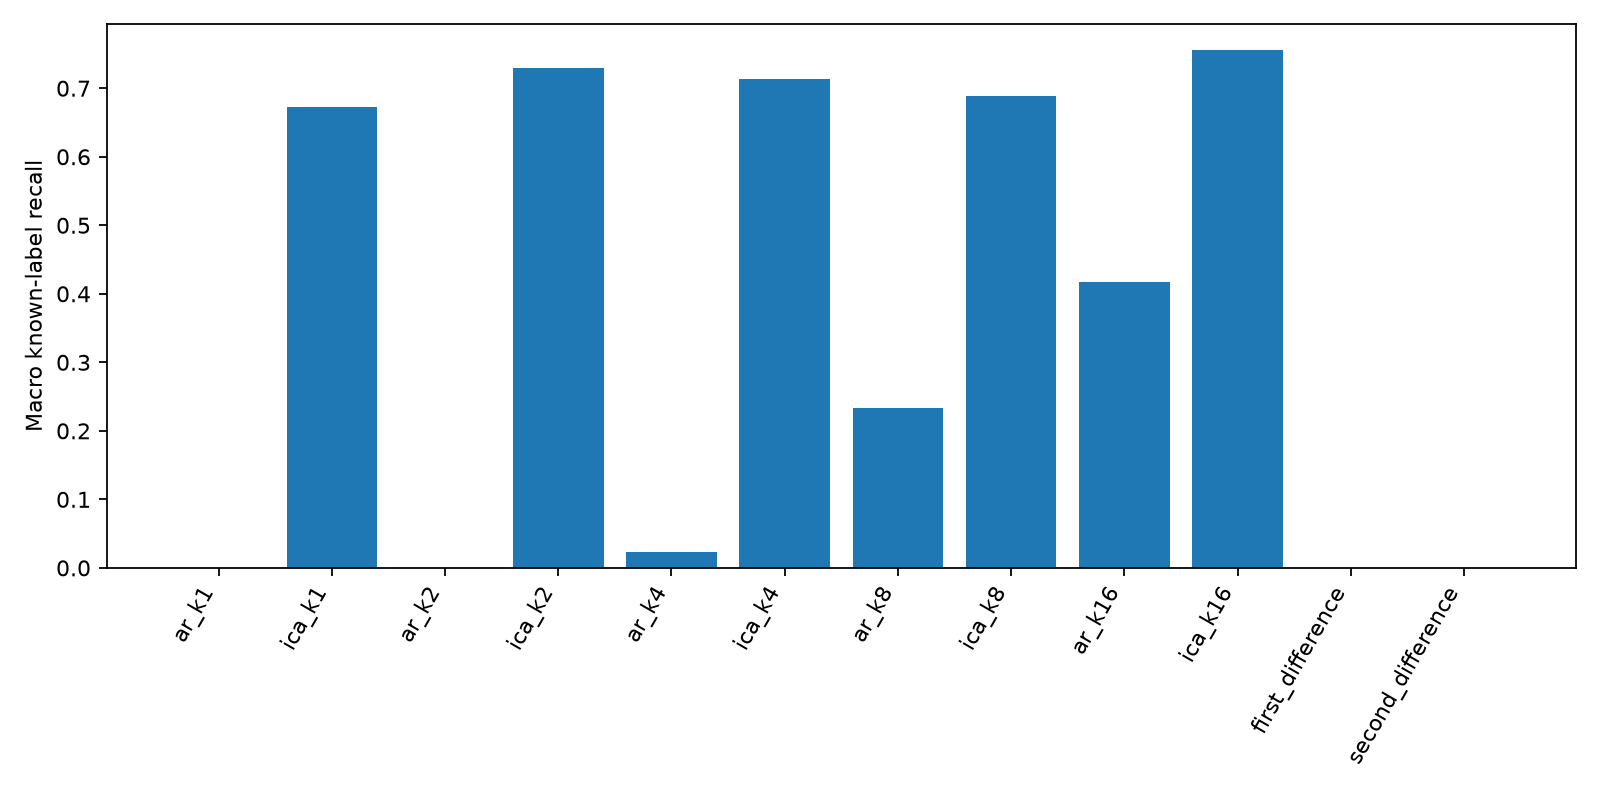
\includegraphics[width=.86\linewidth]{heldout_detection_comparison.png}
  \caption{Known-positive macro recall and candidate counts at the quiet-calibrated operating points. The unequal candidate budgets are scientifically consequential.}
  \label{fig:detection}
\end{figure}

\subsection{Why the positive quiet-$z$ field appears unexpectedly clean}
The visual change is consistent with a compound normalization effect. Stable anatomical brightness contributes strongly to the signed FIR output because the kernel has positive DC gain, but it is subsequently removed by the pixel's own quiet median. Rapid noise is partly averaged by the nine-frame kernel, whereas persistent calcium-like excursions add constructively. Dividing by robust local quiet variability then promotes changes at stable pixels and discounts chronically noisy pixels. Finally, rectification maps every sub-baseline value to black. These mechanisms predict a sparse, high-contrast display even if the ICA kernel itself is replaceable by an ordinary smoother.

\begin{figure}[t]
  \centering
  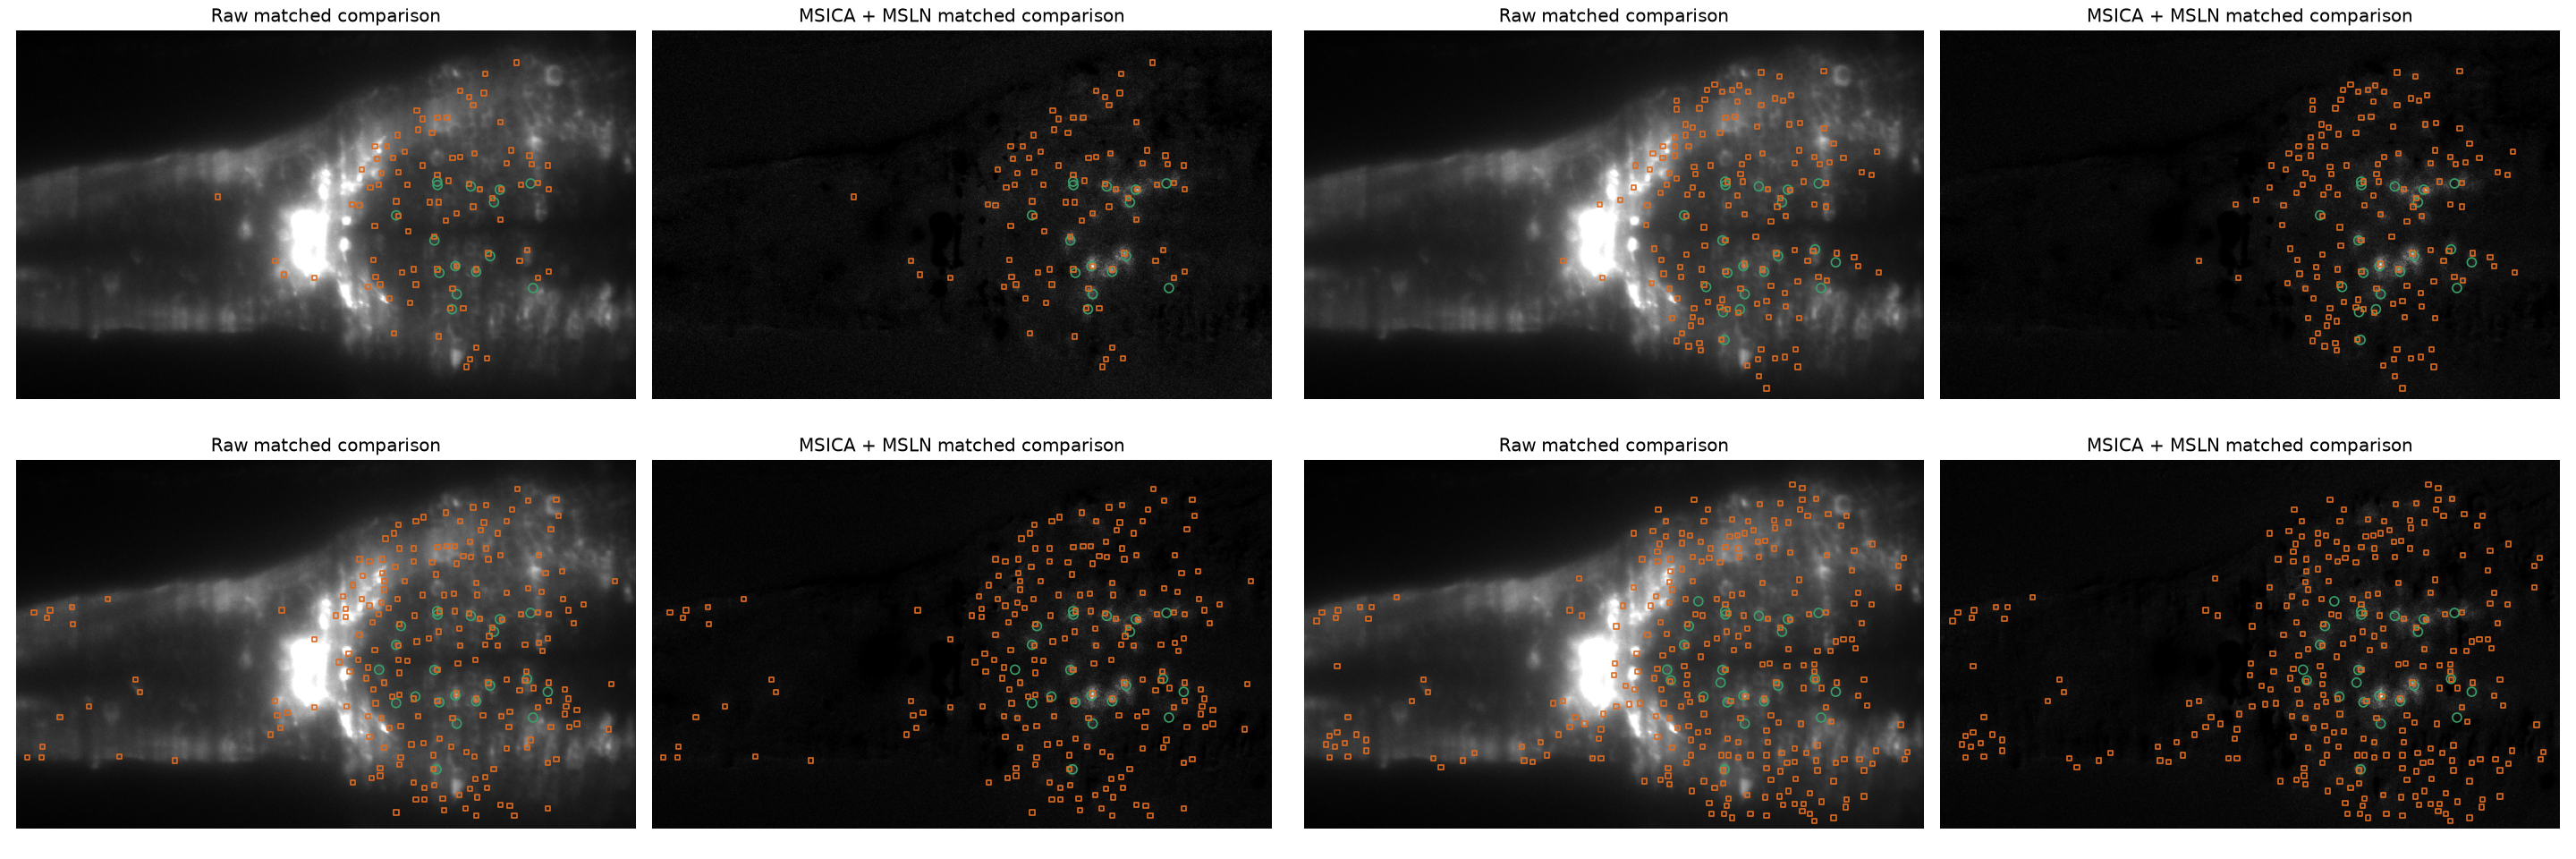
\includegraphics[width=\linewidth]{spatial_overview.png}
  \caption{Four-burst audit overview. Green circles are sparse expert annotations and orange squares are candidates from the frozen label-free $K=8$ lane. Grayscale backgrounds prevent evidence color from being confused with annotations. Unmatched candidates remain unknown.}
  \label{fig:spatial}
\end{figure}

\section{Long-history tap sweep}
We next tested physical FIR lengths of 2, 3, 5, 9, 17, 25, 33, 51, 75, 101, 151, and 201 samples (20 ms to 4 s of causal history). Three seeds and four temporal folds were fitted without labels. Full-rank ICA ceased to be reliable as dimensionality grew: 15/15 fits converged at 2--5 taps, 14/15 at 9, 10/15 at 17 and 25, 2/15 at 33, and 0/15 at every length from 51 through 201. Median conditioning worsened from 130 at two taps to 23,150 at 201 taps, while long-kernel cross-fold cosine similarity was only 0.04--0.09. More unconstrained taps therefore supplied degrees of freedom without supplying an identifiable temporal operator.

To test long physical history without the same parameter explosion, a pre-label amendment represented 51--201 physical taps in low-frequency discrete-cosine bases of rank 8, 16, or 32. A stability gate froze the 201-tap, rank-8 DCT--ICA kernel before label evaluation. The learned kernel was a smooth, six-zero-crossing oscillatory band-pass-like operator: its peak response was 0.75 Hz, while its DC gain was only 0.027. It is not a finer moving-average estimate and should not be interpreted as one.

\begin{figure}[t]
  \centering
  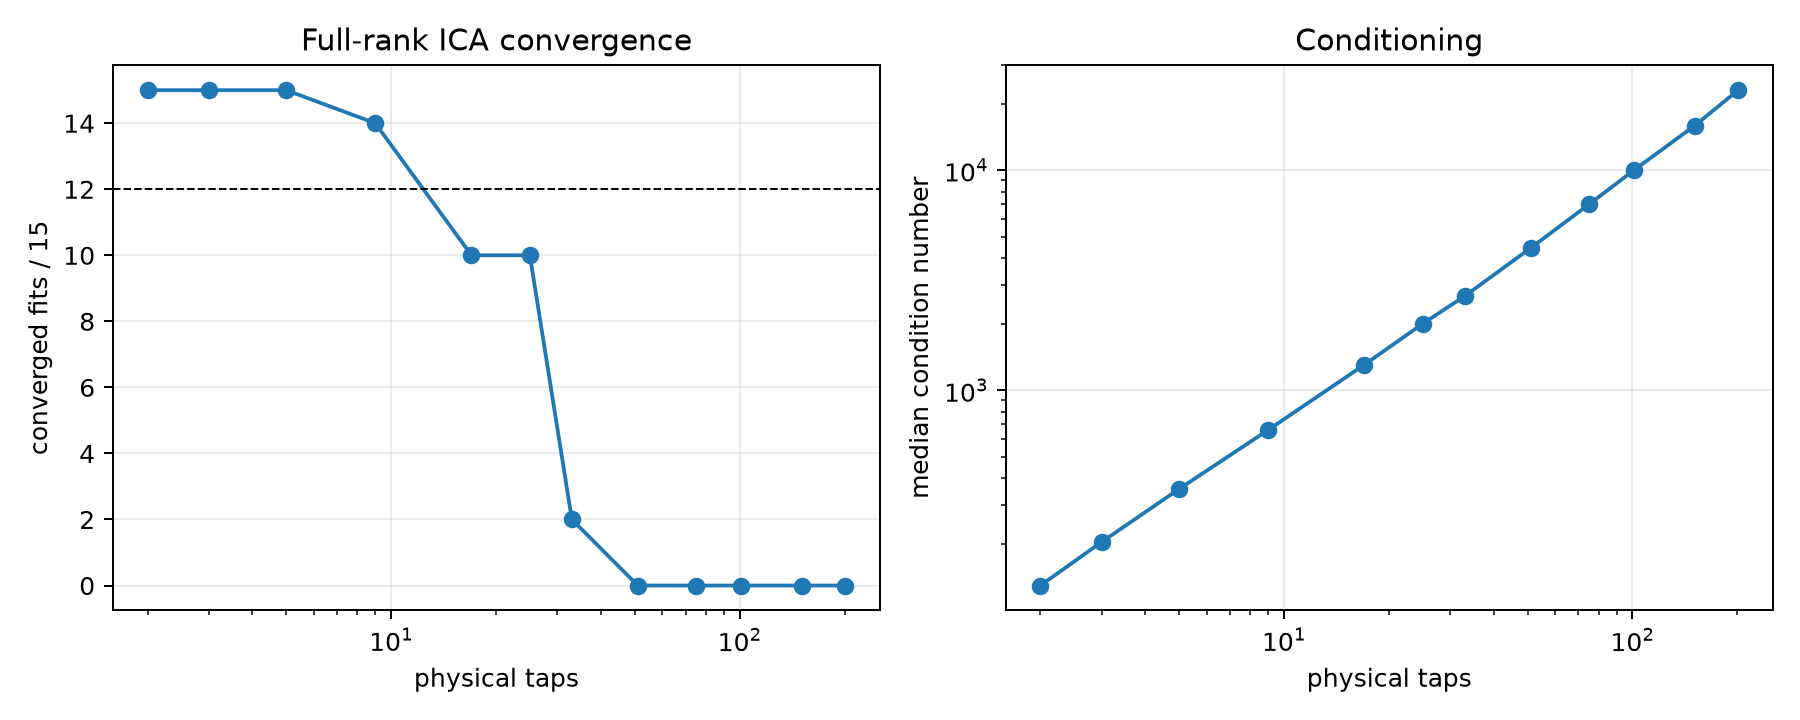
\includegraphics[width=.92\linewidth]{long_history_stability.png}
  \caption{Full-rank temporal ICA loses convergence and becomes progressively ill-conditioned as the number of physical taps increases. The dashed line denotes 12/15 converged fits.}
  \label{fig:long-stability}
\end{figure}

\begin{figure}[t]
  \centering
  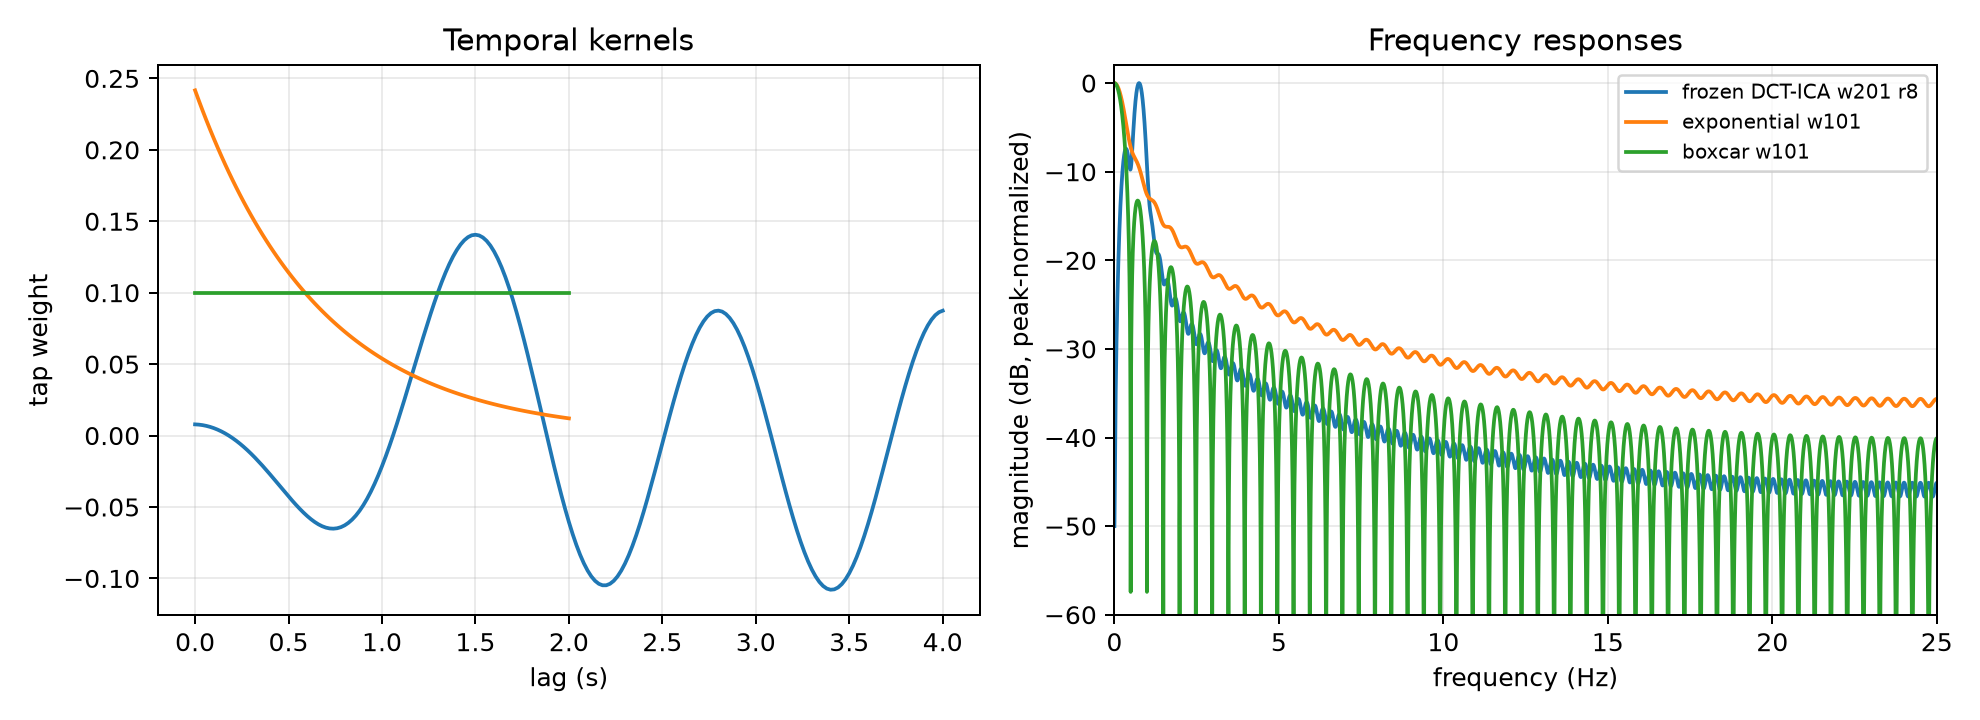
\includegraphics[width=.95\linewidth]{long_history_frequency.png}
  \caption{The frozen 201-tap rank-8 DCT--ICA kernel compared with deterministic 101-tap controls. The learned long-history kernel peaks near 0.75 Hz and strongly suppresses DC; exponential and boxcar controls are ordinary low-pass integrators.}
  \label{fig:long-frequency}
\end{figure}

At its label-free quiet-calibrated operating point, the frozen long-history lane recovered 36/79 known occurrences with 700 candidates (macro recall 0.4205). Its burst recalls were 0.133, 0, 0.810, and 0.739, revealing severe temporal nonstationarity. The post-hoc operating-point winner, a 101-tap exponential smoother, recovered 73/79 but emitted 1,950 candidates and therefore cannot be called more precise. At matched low candidate budgets, 17-tap full-rank ICA was best: it recovered 48, 55, and 56 known occurrences at budgets of 20, 40, and 60 candidates per burst. At budgets of 100 and 150, a five-tap exponential was best (64 and 66 matches). Thus the data reject the hypothesis that at least 100 freely learned weights are required merely because the recording rate is 50 Hz. Tap count defines history duration, but frequency resolution and meaningful identifiability also depend on basis constraints, sample support, stationarity, and the evaluation budget.

\begin{figure}[t]
  \centering
  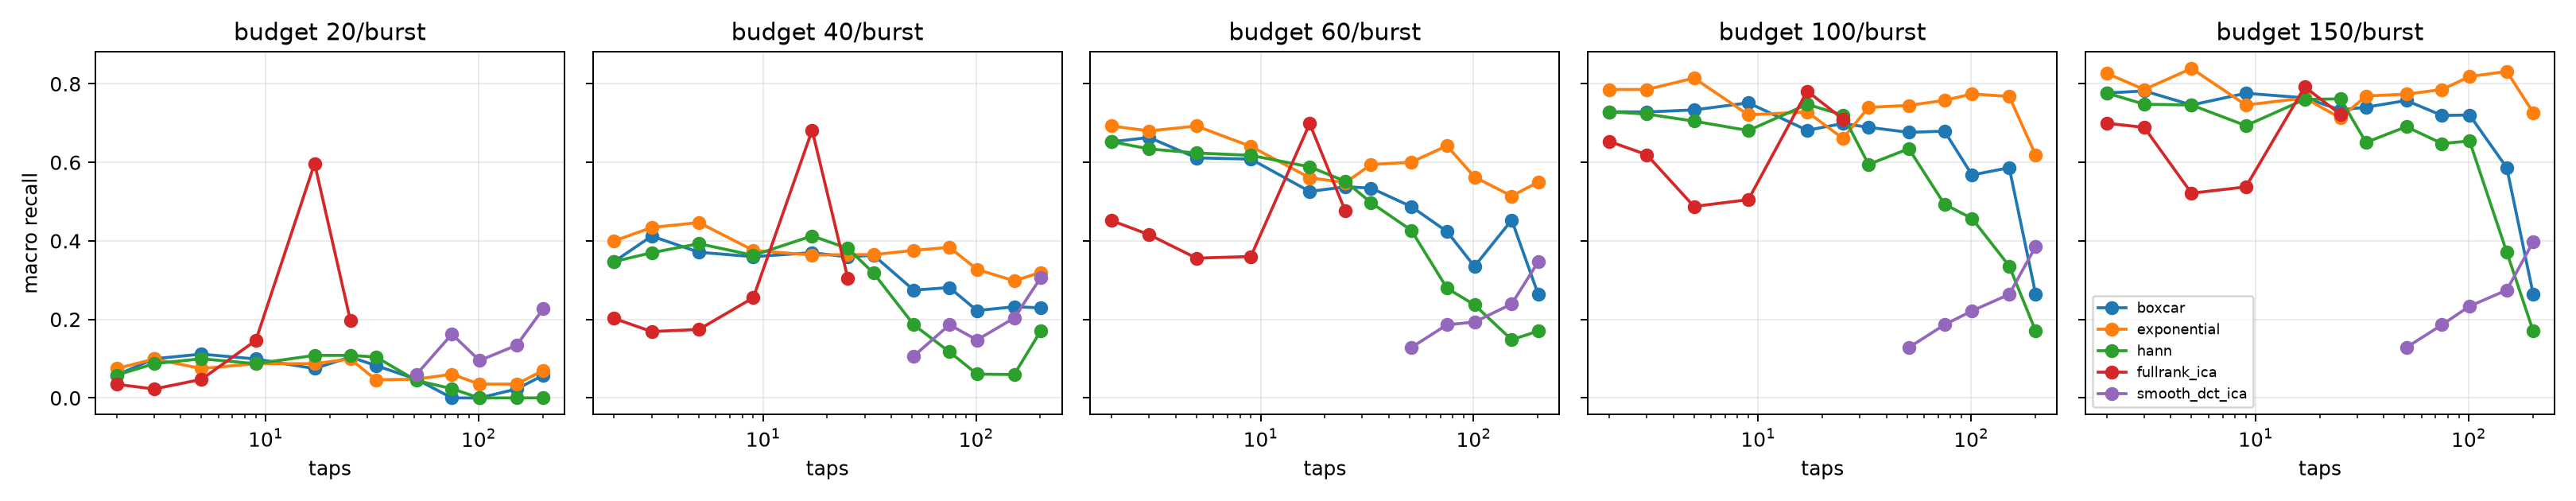
\includegraphics[width=\linewidth]{long_history_fixed_budget.png}
  \caption{Known-positive macro recall at fixed candidate budgets per burst. The rank-8 DCT--ICA curves are shown for the smooth-basis family. Short ICA dominates the low-budget regime; long deterministic smoothing does not dominate until permissive budgets.}
  \label{fig:long-budget}
\end{figure}

The long-history experiment narrows the interpretation of the visually clean positive quiet-$z$ field. Robust pixelwise normalization and rectification remain valuable, but long unconstrained ICA does not expose a progressively clearer physiological timescale. A more defensible next model would estimate a small number of interpretable time constants or a regularized low-order basis, preregistered against matched-budget controls, rather than learning one independent coefficient per 20 ms sample.


\section{Critical controls and next experiments}
After the pending human and exhaustive-annotation gates are satisfied, the
primary mechanistic experiment should factor temporal operator from
normalization while keeping candidate selection and evaluation identical:
\begin{enumerate}
\item raw intensity with and without pixelwise quiet-$z$;
\item uniform nine-frame moving average with quiet-$z$;
\item normalized copies of the learned $K=8$ FIR: unit $\ell_2$ norm (current), unit DC gain, and matched equivalent noise bandwidth;
\item quiet-fitted PCA low-frequency component with quiet-$z$;
\item the learned $K=8$ ICA FIR with global rather than pixelwise quiet normalization;
\item the learned FIR without positive rectification, reporting positive and negative excursions separately.
\end{enumerate}
All lanes should be frozen without labels, evaluated at matched candidate budgets and matched quiet false-alarm rates, and compared per burst. Kernel stability should be evaluated across additional quiet samples and seeds. A fixed candidate panel should undergo exhaustive expert review to estimate precision and distinguish neural signal, motion, vascular structure, and illumination artifacts. These controls determine whether ICA contributes beyond robust temporal integration and whether the visually clean field reflects biological specificity.

\section{Staged research program after the long-history benchmark}
\label{sec:research-program}

The long-history study changes the research objective. The immediate problem
is no longer finding a temporal lane with high known-positive recall; it is
determining whether compact candidates are biologically correct at scarce
review budgets. Sparse-positive labels cannot classify unmatched detections,
so candidate count is only selectivity pressure. The next program therefore
places a bounded truth-set and blinded candidate adjudication before any new
model search.

\subsection{Evidence-constrained working model}

Across the completed studies, useful gains repeatedly arise from short temporal
integration, robust per-pixel quiet normalization, and local spatial context.
Increasing model freedom has not produced equally stable evidence. Table
\ref{tab:frontier} summarizes the landmarks that constrain the next decisions;
rows use different carriers and operating-point contracts and are not a
leaderboard.

\begin{table}[t]
\centering
\small
\caption{Decision landmarks after the temporal and spatial audits. ``B'' is
the candidate budget per burst. Unmatched candidates remain unknown.}
\label{tab:frontier}
\begin{tabular}{p{.24\linewidth}p{.42\linewidth}p{.25\linewidth}}
\toprule
Finding & Evidence & Decision \\
\midrule
Compact temporal ICA & \texttt{fullrank\_ica\_w17} recovered 48/79, 55/79,
and 56/79 at B20, B40, and B60 & Primary compact temporal candidate \\
Deterministic integration & \texttt{exponential\_w5} recovered 55/79 at B60
and 64/79 at B100 & Primary simple comparator \\
Long temporal ICA & Full-rank fits had 0/15 convergence at every 51--201 tap
length; frozen DCT--ICA recovered 36/79 with 700 candidates & Stop long free-tap
sweeps \\
Local coherence & Family-frozen \texttt{coherence\_w15} recovered 48/79 at
B20 versus 43/79 for its carrier and improved all four bursts & Compact spatial
confirmation candidate \\
Latent dynamics & Offline smoother amplitude recovered 55/79 with 320
candidates and won all four bursts & Noncausal ceiling; preservation gates
remain incomplete \\
Model expansion & A bounded linear ranker tied a residual MLP; protected
quantization and hard pooling did not improve the reference & Do not widen MLP,
quantization, or global-fusion grids \\
\bottomrule
\end{tabular}
\end{table}

The central falsifiable hypothesis is that the apparent temporal-ICA advantage
can largely be explained by an ordinary short integrator followed by quiet
normalization. A second hypothesis is that causal neighborhood coherence adds
orthogonal information at the top of the candidate list. The program must also
remain open to a third outcome: many apparent false positives may be real but
previously unlabeled neurons.

\subsection{Estimands and protected endpoints}

The legacy 79 occurrences support known-positive recall at fixed budgets, not
ordinary precision. A new exhaustive region must support object- and event-
level precision--recall curves, average precision (AP), precision at fixed
recall, false events per field-minute, centroid/footprint error, duplicate,
split, and merge rates, and calibration with abstention. Peak amplitude,
temporal area, onset/peak timing, and trace shape remain separate scientific-
signal guards.

Budgets 20 and 40 per burst are primary because they represent scarce review
attention; budget 58 is secondary and budgets 80 and 100 are screening
endpoints. Uncertainty is grouped by recurring ROI identity and burst. Adjacent
frames are not treated as independent observations. Lane definitions,
normalization, temporal pooling, NMS, matching, ranking ties, and analysis code
are frozen before protected labels are opened.

\subsection{Gate 0: finish the existing hard-observation review}

The detector-blinded materials for 25 observations are already available under
\path{Outputs/HardROIAdjudication/}. All rows for ROI 007, 008, 010, 014, 015,
017, 019, 020, and 023 must receive a final anatomical/activity disposition,
canonical identity, morphology/context, reviewer provenance, and a complete
onset--peak--end triple whenever timing changes. Only rows explicitly marked
\texttt{adjudicated} enter the non-provisional exact CPU re-score.

This gate can clarify identity conflicts, temporal misses, localization misses,
NMS suppression, and proposal misses. It cannot estimate precision because the
panel was selected from known difficult observations.

\subsection{Experiment 1: bounded exhaustive truth and stored-candidate test}

\paragraph{Region design.}
Select one morphology-rich calibration tile and one non-overlapping protected
tile in the anatomically relevant right field. The calibration tile may include
known hard identities, but that enrichment is recorded. The protected tile is
chosen with a deterministic seed from a label-free tissue/quality mask, without
detector scores or known-label outcomes. A raw-only pilot estimates reviewer
minutes; final tile dimensions, expected to be approximately 96--128 pixels per
side, are frozen from anatomy, visibility, and workload alone.

\paragraph{Blinded review.}
First review synchronized raw, fixed positive-change, and trace views without
model markers. Mark every visible object/event. Next reveal a randomized,
model-blinded union of frozen candidates to catch omissions. Re-review all
unresolved examples and at least 20\% of accepted/rejected examples after a
washout period or with a second reviewer. Each object receives a persistent
identity and footprint; each event separately records neuron, artifact,
background, or unresolved status, center/membrane morphology,
isolated/crowded context, visibility, timing, and motion/illumination/vascular
flags. Coverage masks are explicit.

\paragraph{Stored temporal disagreement.}
Before fitting a new model, use the completed long-history scores to compare
\texttt{fullrank\_ica\_w17} and \texttt{exponential\_w5}. Freeze the common set,
each lane's unique candidates, a Raw Direct reference, and a raw-discovery
sample at B20, B40, B60, and B100. Candidate order is randomized and lane
identity hidden. The primary comparison is exhaustive-region AP and precision
at matched recall; sparse-label recovery is secondary.

A provisional preregistration target is an AP gain of at least 0.03 plus a
precision-at-matched-recall gain of at least 0.05, without material loss in
three or more bursts. The exact thresholds must be frozen before protected
review and accompanied by grouped intervals and raw paired disagreements. If
the lanes are practically equivalent, the deterministic exponential is
preferred for simplicity and streaming reliability.

\subsection{Experiment 2: unified compact causal confirmation}

After the truth gate, evaluate a single prespecified panel under identical
carrier, temporal-pooling, candidate, NMS, matching, and budget semantics:

\begin{enumerate}
  \item Raw Direct;
  \item the frozen quiet-standardized carrier;
  \item \texttt{fullrank\_ica\_w17} with positive per-pixel quiet
        normalization;
  \item \texttt{exponential\_w5} with the identical normalization;
  \item \texttt{coherence\_w15} under its frozen carrier semantics;
  \item standalone \texttt{propagation\_lag2\_w15}, described as temporal
        recurrence rather than causal biological propagation;
  \item causal latent-filter amplitude under the frozen state model.
\end{enumerate}

The offline RTS smoother is a noncausal ceiling, not a promotable lane. Float
global normalization remains a visualization transform; its post-hoc
temperature/pooling ceiling does not enter primary selection.

If the temporal comparison remains unresolved, use a small mechanism
factorial: identity, five-frame boxcar, five-frame exponential, and frozen
17-tap ICA, each with global robust or per-pixel quiet robust normalization.
Positive-only versus two-sided scoring is added only for the two finalists.
This isolates operator and normalization effects without another kernel search.

The comparison hierarchy is temporal ICA versus exponential, survivor versus
the carrier, and then prespecified coherence and recurrence additions. A lane
advances only if it improves exhaustive-region AP/precision; recovers at least
four additional known occurrences at B20 or B40 with non-worse behavior in at
least three bursts unless the exhaustive endpoint supplies the stronger
predeclared decision; preserves amplitude, area, and timing; remains stable to
ROI-grouped resampling and nearby NMS radii; and completes the required
three-section scientific audit. A null result freezes the simplest baseline
and stops model expansion.

\subsection{Conditional Experiment 3 branches}

Only the branch earned by Experiment 2 should run first.

\paragraph{Interpretable time constants.}
If a temporal integrator wins, replace a free coefficient per frame with a
small nonnegative bank of fixed causal exponentials, for example 40, 80, 160,
320, 640, and 1280 ms, plus a simplex-constrained mixture. Compare the
individual filters and mixture with the frozen five-frame exponential,
17-tap ICA, boxcar controls, causal latent amplitude, and the smoother ceiling.
Reject the branch if selected weights vary across temporal folds, gains appear
only at permissive budgets, or timing exceeds the signal guard.

\paragraph{Morphology-conditional ranking.}
If coherence or recurrence wins and exhaustive negatives exist, retain the
carrier as an immutable skip and fit only a bounded linear model, a monotone
additive model, and at most one center-versus-membrane gate. Inputs are limited
to coherence, recurrence, center/annulus response, cross-scale agreement,
crowding, and an artifact/motion flag. Optimize AP and B20/B40 ordering on the
calibration region with burst and identity grouping, then open the protected
region once. Stop if gains occur only at B58, if the gate tracks acquisition
field rather than morphology, or if one frozen feature is equivalent.

\paragraph{Causal rise/decay dynamics.}
If the smoother remains a useful ceiling and the causal filter approaches it,
test one compact rise/decay or innovation-gated state model against the frozen
scalar AR(1), not a broad Kalman grid. Preserve the raw/quiet-standardized trace
as a skip. Require perturbation stability, amplitude/area preservation, peak
error no greater than one frame, and measured causal latency.

\subsection{Independent recording and streaming gates}

A general detector claim requires at least one recording excluded from fitting,
family selection, thresholding, reviewer training, and figure selection. The
exact finalist, two baselines, preprocessing, field boundaries, quiet-window
rules, budgets, calibration, abstention, and audit manifest are frozen before
opening confirmation labels. Split by fish where possible and session/day
otherwise; a held-out interval from the present movie is not an independent
recording.

Only a method that passes this gate enters a frame-by-frame benchmark. Measure
p50/p95/p99 end-to-end latency, peak RSS/VRAM, warm-up, missed-frame behavior,
checkpoint recovery, and fallback output. The target is p99 below the 20 ms
frame period, with a p95 target below 15 ms for headroom. An offline method must
retain a simpler causal fallback.

\subsection{Resource-bounded PC schedule}

The planning snapshot on 2026-08-12 recorded a 24-core/32-thread Intel
i9-14900K, 78 GiB RAM with 58 GiB available, an RTX 4070 SUPER with 12,282 MiB
VRAM, and approximately 1.8 TiB free disk. The GPU was active, so the snapshot
did not authorize a run. The prior long-history numerical stage completed 57
detection lanes in 675.9 s; the feature audit used 232.5 s and 4.4 GiB peak
RSS. Completed audited roots were approximately 0.8 GiB, but media rendering
can dominate time because an audit may contain hundreds of videos.

\begin{table}[t]
\centering
\small
\caption{Serial execution queue. Time ranges are planning envelopes and are
replaced by smoke-run extrapolation before launch. Every computational run
requires explicit user selection.}
\label{tab:pc-schedule}
\begin{tabular}{p{.11\linewidth}p{.30\linewidth}p{.20\linewidth}p{.27\linewidth}}
\toprule
Order & Work & Envelope & Resource policy \\
\midrule
Q0--Q1 & Freeze manifests; finish hard-observation review & Human-gated & No
heavy compute \\
Q2--Q4 & Truth-set pilot, stored panel assembly, blinded review & 15--45 min
compute plus reviewer time & Two CPU threads; one encoder \\
Q5 & Compact smoke and ETA calibration & 15--30 min & Serial chunks; bounded
GPU only if required \\
Q6 & Unified numerical confirmation & Target $<60$ min before audit & One
process; checkpoint by burst/fold \\
Q7 & Full scientific-audit media & Reserve 1--3 h and at least 5 GiB & One
encoder; no fitting overlap \\
Q8--Q9 & One earned branch; independent confirmation & Re-estimate separately &
Fresh roots and preflights \\
\bottomrule
\end{tabular}
\end{table}

CPU work defaults to two numerical-library threads, one low-priority process,
atomic per-burst/fold checkpoints, and no multiprocessing fan-out. GPU work
defaults to one worker, a 4 GiB allocation cap, at most eight-frame projection
chunks, and CPU-backed output maps. Audit production uses one encoder and
resumable per-ROI media.

Every launch revalidates input hashes and shapes, projection geometry, exact
combination count, output non-collision, git provenance, active processes,
memory, swap, disk, VRAM, and a read-only preflight. The default readiness
thresholds are at least 32 GiB available host memory, less than 0.5 GiB swap in
use, at least 100 GiB free disk plus four times the projected artifact size,
and at least 8 GiB free VRAM with sustained low utilization for GPU work. A
tiny smoke precedes a full run. Heartbeats are written every 30--60 s.

Stop if available RAM falls below 24 GiB, swap exceeds 1 GiB, GPU temperature
remains at or above 80 C for 60 s, an NVIDIA Xid/OOM occurs, a heartbeat stalls
for five minutes, an input digest changes, an output collision appears, or
desktop responsiveness degrades. A stop preserves checkpoints and records the
run as incomplete.

\subsection{Expected outcomes and claims boundary}

The expected, but not assumed, result is that deterministic short integration
will explain much of the temporal-ICA improvement and that coherence or
recurrence will help at tight budgets. If the exponential and ICA lanes are
equivalent, simplicity wins. If 17-tap ICA has a protected low-budget precision
edge, only the interpretable time-constant branch is justified. If spatial
context wins, the next model is a tiny morphology-conditional ranker. If many
unmatched candidates are accepted neurons, the annotation set expands and all
frozen baselines are recomputed. If artifacts dominate, acquisition and
nuisance modeling take priority. If no compact lane passes, the null result
stops local model search and motivates an independent recording.

Until these gates pass, the study does not claim precision, physical source
separation, biological propagation, cross-recording generalization, or
real-time readiness. Longer-term persistent-identity/event inference, domain
calibration, genuine multi-view source separation, left/right intent, and
inverse control remain downstream programs rather than extensions authorized by
this benchmark.

\section{Limitations}
The labels are sparse positives and do not define exhaustive negatives. The same recording supplied quiet fitting and event evaluation, although labels were withheld during fitting. Temporal lags are pseudo-channels from one camera, so ICA identifiability arguments for independent sensors do not directly apply. The selected $K=8$ kernel has moderately high, not perfect, seed stability and a condition number of 1192. Visual sparsity is enhanced by rectification and display scaling. No causal biological propagation, motion invariance, cross-recording generalization, or precision claim is established.

\section{Reproducibility and provenance}
The numerical run and scientific audit are stored under
\texttt{Outputs/TemporalIdentification/spon\_ca\_burst\_multilag\_temporal\_identification\_v1}.
The numerical computation completed in 47.9 seconds using two CPU threads. The audit contains one expert-only and one model-only full-field video, 27 expert close-ups and traces, 398 consolidated model close-ups and traces, and 79 nearest-candidate comparison traces. All 427 videos passed full decoding, frame-count, duration, dimension, and section-specific annotation-color validation. The frozen audit lane is \texttt{ica\_k8}; \texttt{ica\_k16} is explicitly recorded as post-hoc.

\section{Living-paper checklist}
\begin{itemize}
\item[$\square$] Add authors, affiliations, imaging preparation, acquisition hardware, and biological protocol.
\item[$\square$] Finalize the existing 25-observation blinded hard-ROI review and exact re-score.
\item[$\square$] Create calibration and protected exhaustive-review regions with explicit coverage.
\item[$\square$] Adjudicate the stored 17-tap ICA versus five-tap exponential disagreement panel.
\item[$\square$] Run the factorial temporal-operator/normalization control study.
\item[$\square$] Add matched-budget and matched-quiet-false-alarm comparisons with confidence intervals.
\item[$\square$] Complete exhaustive review of a frozen candidate panel and report precision.
\item[$\square$] Test at least one independent recording or a preregistered held-out interval.
\item[$\square$] Add motion and illumination covariates and artifact-stratified analysis.
\item[$\square$] Decide final terminology after determining whether ICA adds value beyond smoothing.
\end{itemize}

\end{document}
